%!TEX root = main.tex

\begin{figure}[tb]
	\centering
%	\newcommand\myheight{0.125}
	\newcommand\myheight{0.171}
	\subfloat[] {
		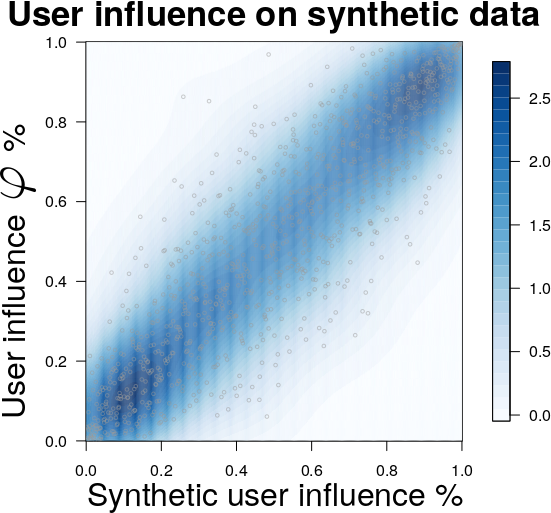
\includegraphics[height=\myheight\textheight]{synthetic-user-influence}
		\label{subfig:artificial-compare}
	}
	\subfloat[] {
		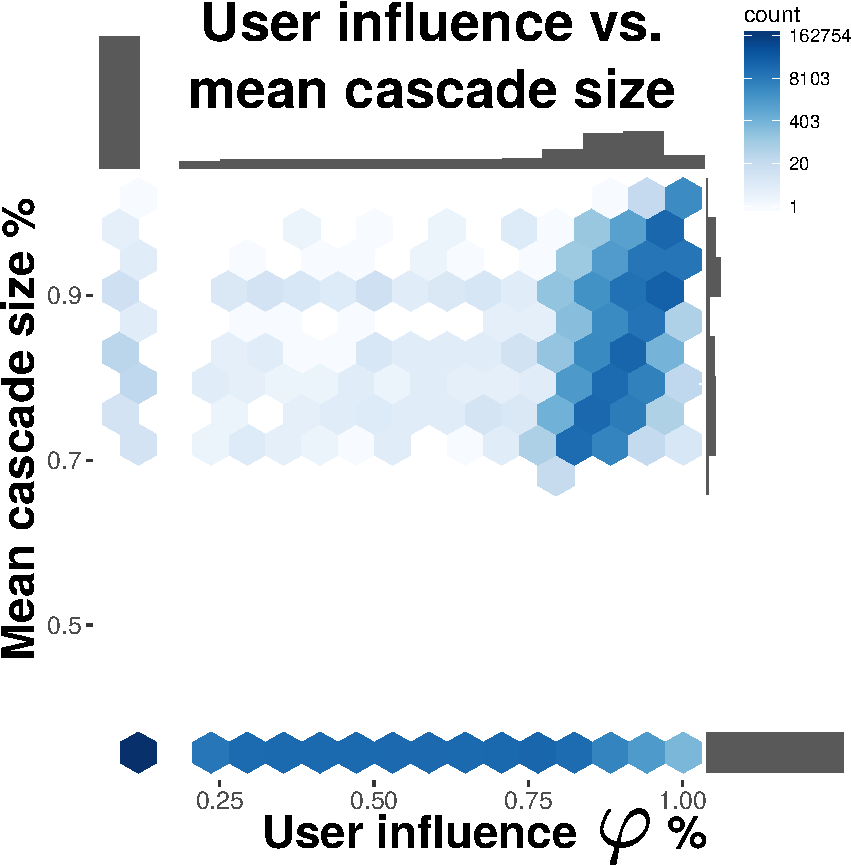
\includegraphics[height=\myheight\textheight]{influence-vs-mcsize}
		\label{subfig:mean-cascade-size}
	}\\
	\subfloat[] {
		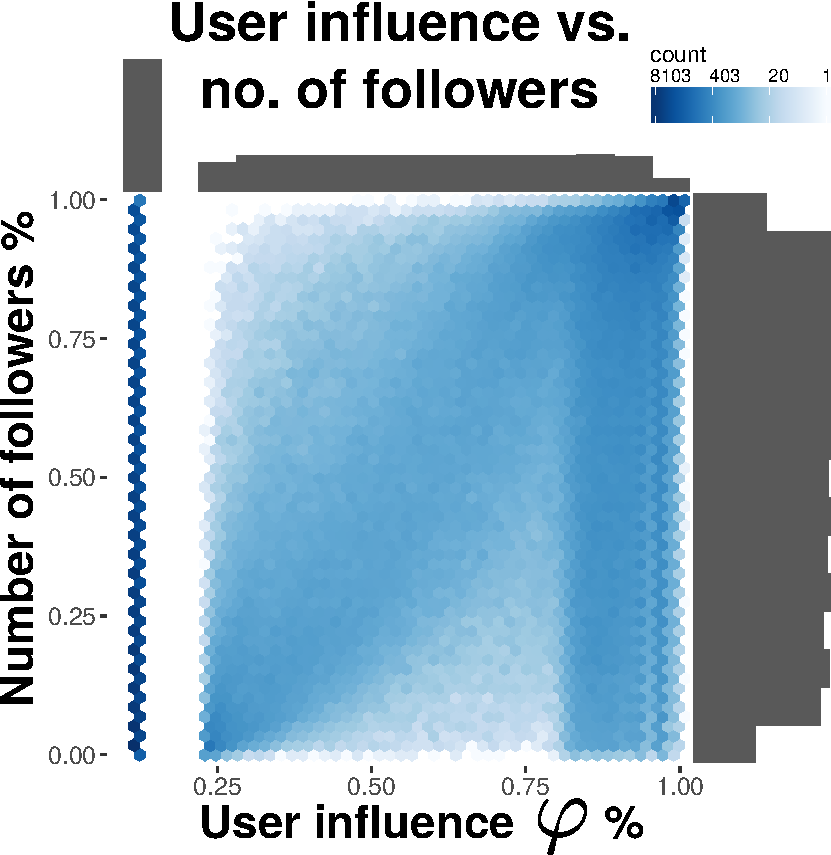
\includegraphics[height=0.19\textheight]{influence-vs-followersCount}
		\label{subfig:no-followers}
	}
%	\subfloat[] {
%		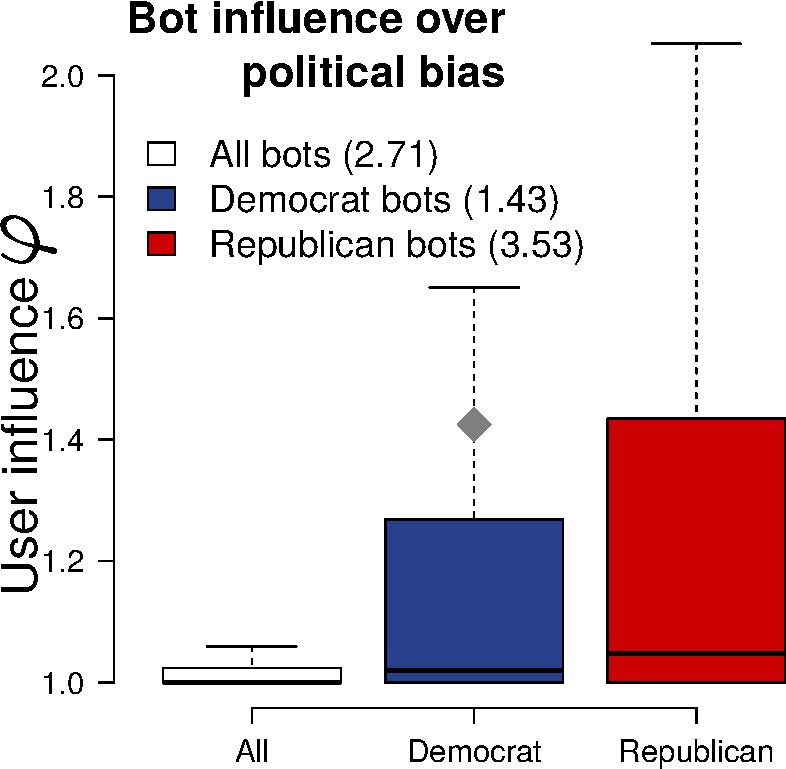
\includegraphics[height=\myheight\textheight]{BOTS_boxplot-influence-vs-political-bias}
%	}
	\caption{ 
		Evaluation of the user influence measure.
		\textbf{(a)} 2D density plot (shades of blue) and scatter-plot (gray circles) of user influence against the ground truth on a synthetic dataset.
		\textbf{(b)(c)} Hexbin plot of user influence percentile (x-axis) against mean cascade size percentile (b) and the number of followers (c) (y-axis) on \debate.
		The color intensity indicates the number of users in each hex bin.
		1D histograms of each axis are shown using gray bars.
		Note $72.3\%$ of all users that initiate cascades are never retweeted.
	}
%	\label{fig:holdout-ll}
%	\captionmoveup
\end{figure}